\section{When Are More Heads Important? The Case of Machine Translation}
\label{sec:anal_mt}

% We focus on the \tfwmt{} model to understand where more attention heads are needed (\S\ref{sec:importance_per_part}), and whether the difference in head importance relates to the sharpness of the attention distribution (\S\ref{sec:important_characteristics}).

% \subsection{When Are More Heads Important?}
\label{sec:importance_per_part}

As shown in Table~\ref{tab:tfwmt_ablation_all_but}, not all \ac{mha} layers can be reduced to a single attention head without significantly impacting performance. To get a better idea of how much each part of the transformer-based translation model relies on multi-headedness, we repeat the heuristic pruning experiment from \S\ref{sec:pruning} for each type of attention separately (Enc-Enc, Enc-Dec, and Dec-Dec).

Figure \ref{fig:componentwise_pruning} shows that performance drops much more rapidly when heads are pruned from the Enc-Dec attention layers. In particular, pruning more than $60\%$ of the Enc-Dec attention heads will result in catastrophic performance degradation, while the encoder and decoder self-attention layers can still produce reasonable translations (with BLEU scores around 30) with only 20\% of the original attention heads. In other words, encoder-decoder attention is much more dependent on multi-headedness than self-attention.

\begin{figure}[!h]
\centering
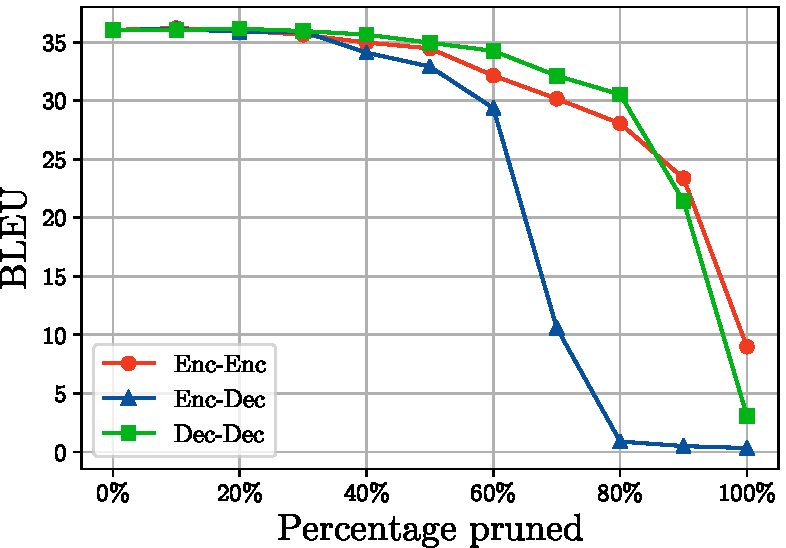
\includegraphics[width=0.6\columnwidth]{img/componentwise_pruning.pdf}
\caption{\label{fig:componentwise_pruning} BLEU when incrementally pruning heads from each attention type in the \tfwmt{} model.}
\end{figure}



\section{Dynamics of Head Importance during Training}
\label{sec:anal_training}

Previous sections tell us that some heads are more important than others in \emph{trained} models. To get more insight into the dynamics of head importance \emph{during training}, we perform the same incremental pruning experiment of \S\ref{sec:incremental_pruning_score} at every epoch. We perform this experiment on a smaller version of \tfwmt{} model (6 layers and 8 heads per layer), trained for German to English translation on the smaller IWSLT 2014 dataset \cite{Cettolo2015ReportOT}. We refer to this model as \textbf{\tfiwslt{}}.

Figure \ref{fig:perf_pruned_per_epoch} reports, for each level of pruning (by increments of 10\% --- 0\% corresponding to the original model), the evolution of the model's score (on \texttt{newstest2013}) for each epoch. For better readability we display epochs on a logarithmic scale, and only report scores every 5 epochs after the 10th). To make scores comparable across epochs, the Y axis reports the relative degradation of BLEU score with respect to the un-pruned model at each epoch.
Notably, we find that there are two distinct regimes: in very early epochs (especially 1 and 2), performance decreases linearly with the pruning percentage, \ie{} the relative decrease in performance is independent from $I_h$, indicating that most heads are more or less equally important. From epoch 10 onwards, there is a concentration of unimportant heads that can be pruned while staying within $85-90\%$ of the original BLEU score (up to $~40\%$ of total heads). 
%When pruning larger quantities of attention heads ($50\%$ or more), important heads are inevitably disabled as well, causing a dramatic drop in performance.

This suggests that the important heads are determined early (but not immediately) during the training process. The two
phases of training are reminiscent of the analysis by \citet{ShwartzZiv2017OpeningTB}, according to which the training of neural networks decomposes into an ``empirical risk minimization'' phase, where the model maximizes the mutual information of its intermediate representations with the labels, and a ``compression'' phase where the mutual information with the input is minimized. A more principled investigation of this phenomenon is left to future work.

% \begin{figure*}[!t]
% \centering
% \begin{subfigure}[c]{0.58\textwidth}
% 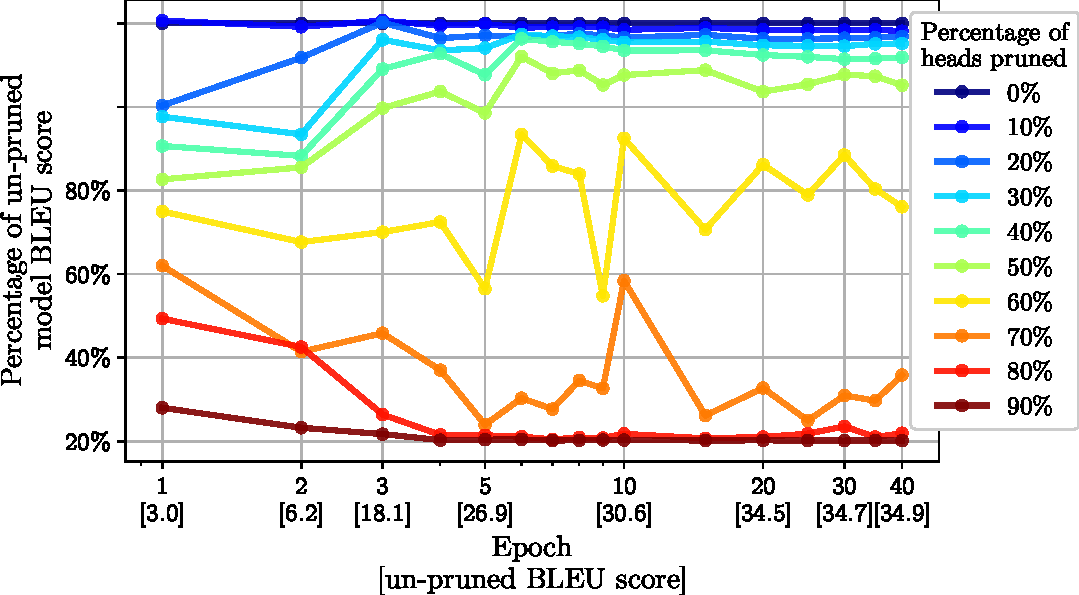
\includegraphics[width=\columnwidth]{img/perf_pruned_per_epoch.pdf}
% \caption{\label{fig:perf_pruned_per_epoch}}
% \end{subfigure}
%          \quad
% \begin{subfigure}[c]{0.3\textwidth}
% 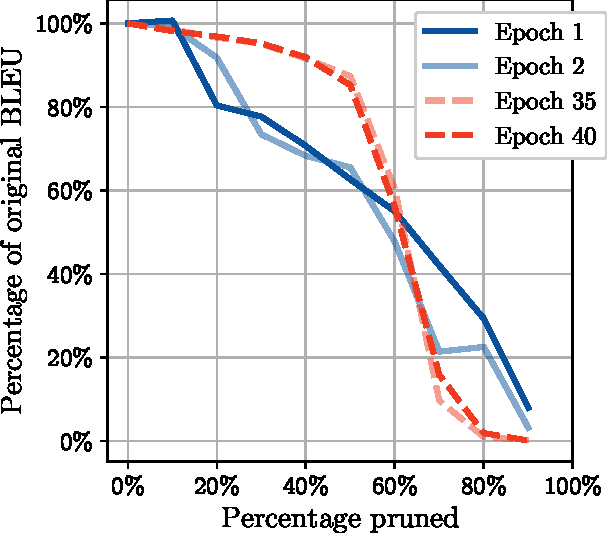
\includegraphics[width=\columnwidth]{img/perf_pruned_per_epoch_extremal.pdf}\caption{\label{fig:perf_pruned_per_epoch_extremal}}
% \end{subfigure}
% \caption{Relationship between percentage of heads pruned and relative score decrease during training of the \tfiwslt{} model. We report epochs on a logarithmic scale. The BLEU score of the original, un-pruned model is indicated in brackets.}
% \end{figure*}
\begin{figure}[t!]
\centering
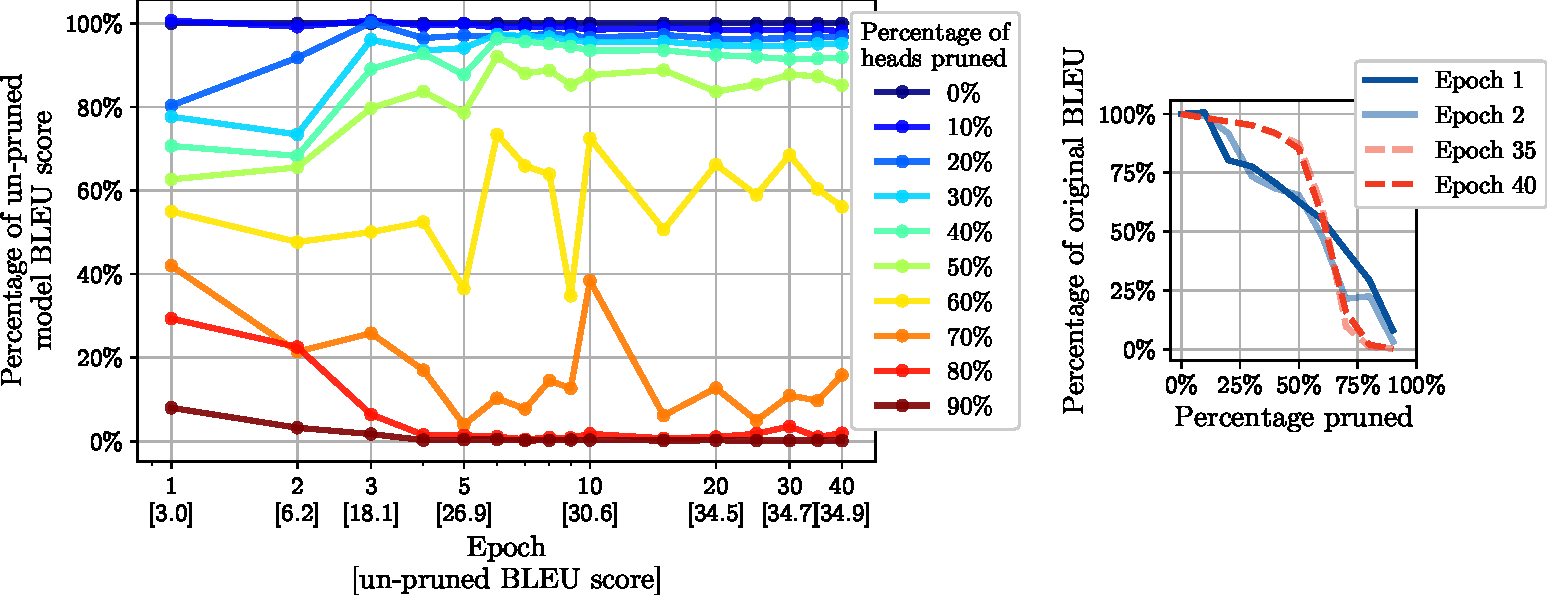
\includegraphics[width=0.95\columnwidth]{img/perf_pruned_per_epoch_both.pdf}
\caption{\label{fig:perf_pruned_per_epoch}\textbf{Left side}: relationship between percentage of heads pruned and relative score decrease during training of the \tfiwslt{} model. We report epochs on a logarithmic scale. The BLEU score of the original, un-pruned model is indicated in brackets. \textbf{Right side}: focus on the difference in behaviour at the beginning (epochs 1 and 2) and end (epochs 35 and 40) of training.}
\end{figure}

% \subsection{Important Heads Tend to be Sharper}
% \label{sec:important_characteristics}

% Finally, we investigate the extent to which the importance of a head relates to the sharpness of its attention distribution.
% First, we say that a head is \emph{important} (or \emph{unimportant}) if it is part of the top 10\% (bottom 10\%) of heads in terms of performance decrease when removed. In other words, important heads are those that cause the biggest drop in performance when they are ablated.
% We then estimate the entropy (averaged over the validation data) of each attention head as a measure of the sharpness of its attention distribution.

%and the \textbf{diversity}, which we define as the smallest KL divergence with any other head in the same layer (both are averaged over the validation data). Intuitively if the diversity of a head $h$ is low, then there exists another head $h'$ in the same layer such that $h$ and $h'$ have very similar attention distributions.
% attention \textbf{distance} (absolute difference between the query position and the position with most attention weight for self-attention layers), attended \textbf{position diversity} (standard deviation of the offset between query position and the position with most attention weight for self-attention layers) and \textbf{attention distribution diversity} (smallest average KL divergence with any other head in the same layer).
% \paul{I had other features based on attention position but I want to double check them. Looks like either there's a bug or a lot of "redundant" heads are attending to the start/end of the sentence only (which would be interesting but I need to confirm)}\paul{}




% Table \ref{tab:crit_comparison} compares the average values of each feature for important and unimportant heads for each type of attention in \tfwmt{}. 
% We observe that, on average, important attention heads tend to have sharper distributions (lower entropy) in the \tfwmt{} model.\footnote{We found that this result did not hold for \bertmnli{}. Largely speaking, the attention distributions in BERT have very low entropy to begin with; perhaps this is a by-product of the extensive pre-training. We leave a more careful investigation to future work.}




% Moreover, it appears that unimportant heads have lower diversity too. This corroborates the conclusions from \citet{li2018multi}, who showed that regularizing for attention diversity improves performance (albeit under a different definition of diversity).

% The results are not so clear-cut for \bertmnli{}. In particular we see that BERT's attention distributions have much higher entropy accross the board. 
%\paul{I can elaborate more here} \gn{If space allows, that might be nice, could also add it as a footnote.} \omer{maybe as a footnote. I think the full stop here is apt.}

% \omer{Can we show this table for BERT as well? We could probably fit them side-by-side if we "smalled" the text.}

% \begin{table}[t]
% \centering
% \setlength\tabcolsep{3pt}
% \begin{tabular}{l|ccc}
%  & Enc-Enc & Enc-Dec & Dec-Dec \\
% \hline\hline
% % Important & 0.90 & 1.27 & 1.09 \\
% % Unimportant & 1.51 & 1.52 & 1.27 \\
% Important & 1.15 & 1.18 & \underline{1.21} \\
% Unimportant &  1.31 & 1.12 & \underline{0.24} \\
% \hline
% \end{tabular}
% \caption{\label{tab:crit_comparison} Average attention entropy for important and unimportant attention heads in \tfwmt{}.}
% \end{table}
